\documentclass[11pt,a4paper]{article}

\usepackage[margin=2.2cm]{geometry}
\usepackage[T1]{fontenc}
\usepackage{lmodern}
\usepackage{booktabs}
\usepackage{graphicx}
\usepackage{float}
\usepackage{caption}
\usepackage{tikz}
\usetikzlibrary{positioning,arrows.meta}
\usepackage[hidelinks]{hyperref}

\setlength{\parskip}{4pt}
\setlength{\parindent}{0pt}
\captionsetup{font=small}

\title{DPDP-Audit: Mid-Submission Report\\[2pt]
\large Checking app privacy policies against app behaviour under India's DPDP Act}
\author{Anurag Kaushal \and Ishaan Giri \and Naveen Mishra \and Nikhil Patidar}
\date{30 October 2026\\[2pt] Covers Stages 1 to 3 (milestones MS-0 to MS-3)}

\begin{document}
\maketitle

\section{Summary}

An app's privacy policy says what personal data it collects, why, and who receives it. The app's
code and its third-party SDKs may do something else. We call such a difference a \emph{compliance
gap}. We study five kinds of gap under India's Digital Personal Data Protection (DPDP) Act, 2023:
undisclosed collection, undisclosed sharing, purpose mismatch, retention mismatch and children's
data.

So far we have:
\begin{itemize}
  \item built a benchmark of 102 app and policy cases whose answers come from fixed rules over
        expert annotations (no LLM in the ground truth), and a 140-case \emph{vagueness ladder};
  \item run two published checkers (PoliCheck and PoliGraph) and three single-prompt LLM baselines;
  \item built DPDP-Audit, an evidence-based review pipeline, in two versions (v1 and v2), with a
        clause tagger fine-tuned with QLoRA;
  \item had two team members check the ladder and a sample of the answer keys by hand.
\end{itemize}

\textbf{Main result.} Our final system (v2 with the fine-tuned tagger) reaches an F1 of 0.705 with a
false-alarm rate of 0.265 on compliant apps. The best baseline, Gemini 3 Flash given the same prompt
as our single-prompt baseline, reaches F1 0.421 but raises an alarm on 97\% of compliant apps. The
published tools reach F1 0.149 (PoliCheck) and 0.166 (PoliGraph). All of v2's gains over the
baselines are statistically significant on every seed.

\textbf{Where the gain comes from.} Baselines built from the pipeline's own parts show what each
layer adds. Rules alone (our tagger and the finder, no LLM) already reach F1 0.524 but raise an
alarm on 91\% of compliant apps. One LLM call that quotes the evidence first and then uses our
decision rules reaches F1 0.557 with 26\% false alarms. The full pipeline adds a further +0.13 to
+0.16 F1 on every seed.

\textbf{What did not work.} The first version (v1) does not beat the single-prompt baseline on F1.
The evidence verifier costs more recall than we allowed, the reviewer agents never used their tools,
and purpose and collection gaps are still mostly missed. Section~\ref{sec:hyp} lists every
hypothesis with its verdict.

\section{Benchmark}

\begin{table}[H]
\centering
\small
\begin{tabular}{p{2.6cm}p{5.4cm}p{6.2cm}}
\toprule
Set & Size & Answer source and status \\
\midrule
Main & 102 cases (34 compliant controls, 68 variants), 118 gold gaps, 433 data flows &
Fixed rules over expert OPP-115 annotations. A hand check of 87 flows found the key wrong on
9 flows (10.3\%). \\
Vagueness ladder & 140 cases: 35 ladders of 4 rungs (clear, explicit, vague, deleted) &
One templated sentence changes per rung. Checked by two members; 110 rungs accepted. \\
Dev splits & 33 + 69 cases from 34 training policies & Same rules. Used only to develop the
pipeline, never for evaluation. \\
\bottomrule
\end{tabular}
\caption{Benchmarks. Cases come from the 35 held-out OPP-115 policies (80/35 split, seed 13).}
\end{table}

Each case has a policy text and an app folder (build file with SDKs, Android manifest with
permissions, and a list of data flows: data type, recipient, purpose and retention). The case
generator is deterministic: running it again gives byte-identical files.

\section{Systems}

\begin{table}[H]
\centering
\small
\begin{tabular}{lp{7.2cm}l}
\toprule
ID & System & Model \\
\midrule
S1 & PoliCheck (authors' code) & rule-based NLP \\
S2 & PoliGraph (authors' released NLP version) & rule-based NLP \\
B1 & One prompt with the raw policy and app files & Qwen2.5-7B \\
B2 & One prompt with exactly the inputs our pipeline gets & Qwen2.5-7B \\
B4 & B2's prompt given to a much stronger model & Gemini 3 Flash \\
v1 & DPDP-Audit as frozen before evaluation & Qwen2.5-3B tagger, 7B reviewers \\
v2 & DPDP-Audit with fixes chosen on the dev splits only (Section~\ref{sec:v2}) & same \\
A1 to A5 & Ablations: verifier off, no retrieval, one generalist reviewer, oracle tagger & same \\
R0 & Rules only: our tagger and the finder, every candidate reported & no LLM \\
B5 & One call over the whole policy, evidence first, then v2's rules and verifier & Qwen2.5-7B \\
B1, B2, B4 sc & Self-consistency: the majority label over the three seeds & as the system \\
\bottomrule
\end{tabular}
\caption{Systems compared. LLM systems run with 3 seeds; the tools and R0 run once. R0, B5 and the
self-consistency baselines were added on 30 October (Section~\ref{sec:parts}).}
\end{table}

\begin{figure}[H]
\centering
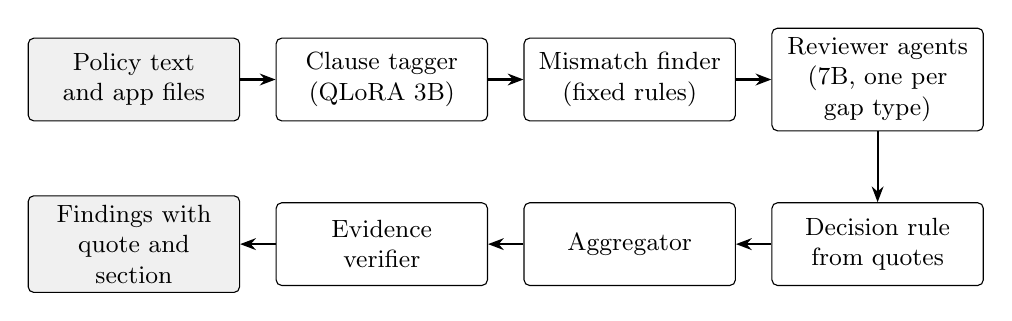
\begin{tikzpicture}[
  box/.style={draw, rounded corners=2pt, align=center, font=\small,
              minimum height=1.05cm, text width=2.45cm, fill=white},
  io/.style={box, fill=gray!12},
  arr/.style={-{Stealth[length=2mm]}, thick},
  node distance=0.45cm]
\node[io] (in) {Policy text\\and app files};
\node[box, right=of in] (tag) {Clause tagger\\(QLoRA 3B)};
\node[box, right=of tag] (find) {Mismatch finder\\(fixed rules)};
\node[box, right=of find] (rev) {Reviewer agents\\(7B, one per\\gap type)};
\node[box, below=0.9cm of rev] (rule) {Decision rule\\from quotes};
\node[box, left=of rule] (agg) {Aggregator};
\node[box, left=of agg] (ver) {Evidence\\verifier};
\node[io, left=of ver] (out) {Findings with\\quote and section};
\draw[arr] (in) -- (tag);
\draw[arr] (tag) -- (find);
\draw[arr] (find) -- (rev);
\draw[arr] (rev) -- (rule);
\draw[arr] (rule) -- (agg);
\draw[arr] (agg) -- (ver);
\draw[arr] (ver) -- (out);
\end{tikzpicture}
\caption{The DPDP-Audit pipeline. The tagger turns each policy paragraph into structured claims.
The finder proposes every flow those claims do not clearly cover. A reviewer copies the policy
sentences that disclose, deny or only vaguely cover the flow. A fixed rule turns the verified
quotes into a gap and its level. The verifier drops findings with a wrong quote or DPDP section and
sends doubtful ones to human review.}
\end{figure}

\section{Results on the main benchmark}

Table~\ref{tab:main} gives the mean over seeds. \emph{Common} keeps only collection and sharing
gaps, which are the gap types the tools model. \emph{Native} uses the tools' own reading, in which a
vague disclosure is not a gap. The false-alarm rate is the share of the 34 compliant apps on which a
system reports any gap.

\begin{table}[H]
\centering
\small
\begin{tabular}{lcccccc}
\toprule
System & F1 & F1 common & F1 native & Label macro-F1 & False alarms & Citation correct \\
\midrule
S1 PoliCheck & 0.149 & 0.186 & 0.192 & 0.225 & 0.912 & by design \\
S2 PoliGraph & 0.166 & 0.212 & 0.079 & 0.197 & 0.853 & by design \\
B1 & 0.182 & 0.183 & 0.246 & 0.177 & 0.971 & 0.325 \\
B2 & 0.181 & 0.176 & 0.206 & 0.107 & 0.745 & 0.894 \\
B4 Gemini 3 Flash & 0.421 & 0.303 & 0.156 & 0.279 & 0.971 & 0.996 \\
v1 (prompted tagger) & 0.186 & 0.156 & 0.114 & 0.353 & \textbf{0.235} & 1.000 \\
v1 (QLoRA tagger) & 0.168 & 0.219 & 0.042 & 0.463 & 0.275 & 1.000 \\
v2 (prompted tagger) & 0.692 & 0.673 & \textbf{0.370} & 0.407 & 0.294 & 1.000 \\
\textbf{v2 (QLoRA tagger)} & \textbf{0.705} & \textbf{0.686} & 0.364 & \textbf{0.495} & 0.265 & 1.000 \\
\bottomrule
\end{tabular}
\caption{Main benchmark, mean over 3 seeds (tools: one run). Pipeline rows use the fixed verifier
(Section~\ref{sec:bug}).}
\label{tab:main}
\end{table}

\begin{figure}[H]
\centering
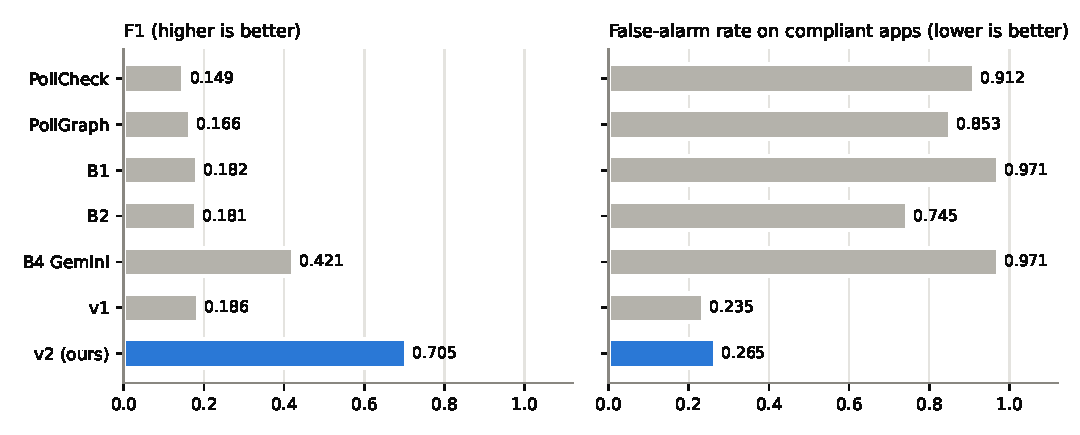
\includegraphics[width=\textwidth]{figures/main_results.pdf}
\caption{F1 and false-alarm rate on the main benchmark (mean over seeds). Only v2 is both accurate
and safe. The stronger model B4 and the rules-only R0 find many gaps but alarm on almost every
compliant app; B5 is safe but finds fewer gaps.}
\end{figure}

Table~\ref{tab:paired} compares systems on the same cases. The 95\% intervals come from a
policy-level bootstrap with 1,000 re-samples, because cases built from the same policy are not
independent.

\begin{table}[H]
\centering
\small
\begin{tabular}{lcc}
\toprule
Comparison (seed 0) & F1 difference & False-alarm difference \\
\midrule
v2 minus B2 & +0.535 [0.451, 0.607] & $-$0.471 [$-$0.706, $-$0.235] \\
v2 minus B4 Gemini & +0.309 [0.235, 0.380] & $-$0.765 [$-$0.912, $-$0.618] \\
v2 minus S1 PoliCheck & +0.574 [0.498, 0.642] & $-$0.706 [$-$0.853, $-$0.558] \\
v2 minus S2 PoliGraph & +0.557 [0.474, 0.629] & $-$0.647 [$-$0.794, $-$0.499] \\
v1 minus B2 & $-$0.024 [$-$0.136, 0.105] & $-$0.471 [$-$0.676, $-$0.265] \\
\bottomrule
\end{tabular}
\caption{Paired differences with 95\% intervals. v2 is the QLoRA-tagger version. Every v2 interval
excludes 0, and the gains over B2, B4 and the tools also hold on seeds 1 and 2.}
\label{tab:paired}
\end{table}

\textbf{Falsifiable claim.} We claimed our system would beat PoliCheck and PoliGraph on their gap
types and B2 on the full benchmark, in both F1 and false-alarm rate. The claim \textbf{fails for v1}
(no F1 gain over B2 or the tools) and \textbf{holds for v2} in every view.

\section{Pipeline v2}
\label{sec:v2}

Our rule is that nothing is tuned on evaluation cases. Every v2 change was found and chosen on the
two dev splits (102 cases from 34 training policies), frozen, and then run once on the main
benchmark and the ladder. The frozen v1 results are kept unchanged and reported next to v2.

\begin{table}[H]
\centering
\small
\begin{tabular}{p{7.4cm}p{7.4cm}}
\toprule
Problem found on the dev splits & Change in v2 \\
\midrule
The verifier's LLM check rejected every correct children's-data and retention finding &
The LLM check is used only for collection and purpose findings; the others keep the rule checks \\
A purpose sentence was rejected when it did not repeat the data type &
It counts when its paragraph names the data type \\
17 of 47 false collection findings came from an 8-paragraph limit &
Up to 16 paragraphs per reviewer, within the same prompt budget \\
A reviewer answering several flows at once often quoted nothing &
One flow per reviewer call \\
The retention reviewer cleared real gaps with unrelated sentences &
A retention quote must be about keeping data \\
\bottomrule
\end{tabular}
\caption{The v2 changes. One more change was tried on dev and rejected because it lowered F1.}
\end{table}

\subsection{The verifier reply bug}
\label{sec:bug}

While reviewing the runs we found that the verifier's reply could not be read in 15\% to 38\% of
pipeline runs: the 7B model wrote one JSON object per finding instead of one list. The code then
kept every finding unchecked. We fixed the reader and re-ran only the verifier on all saved runs.
In the 2,958 re-verified runs every reply is read (14 findings in total got no verdict because the
reply was cut off). All pipeline numbers in this report use the fixed verifier. With the bug, v1
seemed to beat B2 (F1 0.343); that gain came from findings that were never checked.

\section{Baselines from the pipeline's parts}
\label{sec:parts}

To see what each layer of the design adds, we added three baselines on 30 October, each removing
one layer:
\begin{itemize}
  \item \textbf{R0, rules only.} Our QLoRA tagger and the finder; every candidate the finder
        proposes is reported. No LLM call.
  \item \textbf{B5, one call, evidence first.} No tagger, no finder, no specialist reviewers, no
        tools and no retrieval. One call reads the whole policy and quotes the evidence for every
        flow; v2's decision rules, aggregator and verifier then decide. Its prompt was fixed on the
        dev splits before it ran on the main benchmark.
  \item \textbf{Self-consistency.} The majority label over the three seeds of B1, B2 and B4, a fair
        counterpart to our pipeline, which also uses three seeds.
\end{itemize}

\begin{table}[H]
\centering
\small
\begin{tabular}{lccccc}
\toprule
System & F1 & F1 common & Label macro-F1 & False alarms & Citation correct \\
\midrule
R0 rules only (no LLM) & 0.524 & 0.551 & 0.430 & 0.912 & 1.000 \\
R0 with the prompted tagger & 0.374 & 0.308 & 0.367 & 1.000 & 1.000 \\
B5 one call (3 seeds) & 0.557 & 0.423 & 0.206 & 0.255 & 0.350 \\
B1 sc / B2 sc & 0.179 / 0.182 & 0.183 / 0.177 & 0.169 / 0.111 & 0.971 / 0.676 & 0.304 / 0.949 \\
B4 sc & 0.473 & 0.328 & 0.292 & 0.971 & 1.000 \\
\textbf{v2 (QLoRA tagger)} & \textbf{0.705} & \textbf{0.686} & \textbf{0.495} & 0.265 & 1.000 \\
\bottomrule
\end{tabular}
\caption{Baselines from the pipeline's parts on the main benchmark.}
\end{table}

\begin{itemize}
  \item \textbf{Rules alone beat every single-prompt baseline on F1} (R0 minus B2 +0.336
        [0.268, 0.403]; R0 minus B4 +0.110 [0.052, 0.178]) but alarm on 91\% of compliant apps. The
        LLM review and the verifier add +0.199 F1 [0.132, 0.263] and cut false alarms by 0.706
        [0.559, 0.853].
  \item \textbf{Evidence-first review with rule-based decisions gives most of the gain even in one
        call}: B5 minus B2 is +0.384 F1 [0.292, 0.466] with 0.382 fewer false alarms.
  \item \textbf{The full pipeline still adds +0.13 to +0.16 F1 over B5, significantly on every seed}
        (+0.151, +0.133, +0.161), at the same false-alarm rate. Without the finder, B5 sends every
        flow to the model, which marks 234 of the 385 clearly disclosed flows (seed 0) as vague or
        omitted; without the specialists' instructions it often cites the wrong DPDP section
        (citation correct 0.350).
  \item \textbf{Self-consistency does not close the gap}: it changes nothing for B1 and B2 and gives
        B4 +0.058 F1; v2 minus B4 sc is still +0.251 [0.179, 0.320].
\end{itemize}

\section{Ablations}

\begin{table}[H]
\centering
\small
\begin{tabular}{llccl}
\toprule
Config & Change & F1 & False alarms & v2 minus config, F1 (seeds 0 / 1 / 2) \\
\midrule
v2 (QLoRA tagger) & none & 0.705 & 0.265 & \\
A1 & verifier off & 0.609 & 0.647 & +0.111* / +0.103* / +0.075* \\
A2 & no DPDP retrieval & 0.740 & 0.167 & $-$0.012 / $-$0.033 / $-$0.060* \\
A3 & one generalist reviewer & 0.723 & 0.167 & $-$0.013 / $-$0.016 / $-$0.026 \\
A5 & oracle tagger (gold labels) & 0.825 & 0.029 & $-$0.113* / $-$0.112* / $-$0.136* \\
\bottomrule
\end{tabular}
\caption{Ablations of v2, mean over 3 seeds. A star marks an interval that excludes 0.}
\end{table}

\begin{itemize}
  \item The \textbf{verifier} matters on every seed: without it recall rises, but false alarms
        rise from 0.265 to 0.647.
  \item \textbf{Retrieval and specialist reviewers do not help}: without them v2 is as good or
        slightly better. The retrieved DPDP text seems to distract the reviewers.
  \item \textbf{Reading the policy is the main remaining error}: with gold annotations (A5) F1 rises
        by about 0.11. A5 is partly circular, because the answer keys come from the same
        annotations.
\end{itemize}

\section{Vagueness ladder and human checks}

Each ladder keeps one policy and one data flow and changes a single sentence: \emph{clear} (names
the practice), \emph{explicit} (denies it), \emph{vague} (generic wording) or \emph{deleted}
(sentence removed). This isolates the effect of wording.

\textbf{Human check.} Two members checked all 140 rungs independently. They agreed on 107 (76\%,
Cohen's kappa 0.19), then settled all 33 disagreements together. 110 rungs are accepted and scored.
The same two members checked 87 flows of 20 main cases: after settling, the answer key is wrong on
9 flows (10.3\%) in 6 cases. The keys are frozen, so this number estimates the label noise in
Section 4.

\begin{table}[H]
\centering
\small
\begin{tabular}{lccccc}
\toprule
System & Clear & Explicit & Vague & Deleted & Explicit minus vague \\
\midrule
S1 PoliCheck & 0.18 & 0.73 & 0.38 & 0.79 & +0.32 (p = 0.064) \\
S2 PoliGraph & 0.38 & 0.00 & 0.03 & 0.93 & $-$0.04 (p = 1.00) \\
B2 & 0.00 & 0.00 & 1.00 & 0.00 & $-$1.00 \\
R0 rules only & 0.85 & 0.57 & 0.78 & 0.64 & \\
B5 one call & 0.88 & 0.53 & 0.81 & 0.07 & \\
v1 (prompted tagger) & 1.00 & 0.53 & 0.84 & 0.14 & $-$0.29 (p = 0.057) \\
v2 (QLoRA tagger) & 1.00 & 0.77 & 0.88 & 0.14 & $-$0.07 (p = 0.63) \\
\bottomrule
\end{tabular}
\caption{Accuracy of the flow's disclosure label per accepted rung (seed 0). Seeds 1 and 2 give the
same picture.}
\end{table}

\begin{itemize}
  \item Only PoliCheck is less accurate on the vague rung than on the explicit one, and not
        significantly. Our pipeline reads the vague rung as well as or better than the explicit one.
  \item B2 calls every flow ``vague'' on every rung.
  \item The deleted rung is a real pipeline error: v2 often reads leftover generic wording as a
        vague disclosure, where PoliCheck correctly says ``omitted''. R0 reads 64\% of deleted rungs
        correctly, so this over-reading comes from the LLM review step, not from the tagger.
\end{itemize}

\section{Clause tagger}

\begin{table}[H]
\centering
\small
\begin{tabular}{lccc}
\toprule
Tagger & Category macro-F1 & Tuple F1 & Tuple F1 with third party \\
\midrule
PrivBERT, fine-tuned (S3) & 0.779 & & \\
Prompted Qwen2.5-3B, categories only (B3) & 0.388 & & \\
Prompted Qwen2.5-3B, claims (v1 tagger) & 0.311 & 0.179 & 0.053 \\
\textbf{QLoRA Qwen2.5-3B (ours)} & \textbf{0.713} & \textbf{0.479} & \textbf{0.288} \\
PolicyLint, statement extraction (S4) & & 0.106 & 0.085 \\
PoliGraph, statement extraction (S4) & & 0.234 & 0.114 \\
\bottomrule
\end{tabular}
\caption{Tagger results on 1,140 held-out OPP-115 paragraphs. A tuple is (category, data type,
does or does not); the last column adds the third party.}
\end{table}

QLoRA training: 4-bit Qwen2.5-3B-Instruct, rank 16, 2 epochs fixed in advance, 2,426 paragraphs
from 72 training policies, 2.8 hours on one T4 GPU. Our tagger extracts about twice the tuple F1 of
the better published tool and more than doubles the prompted tagger's macro-F1. In the pipeline the
gain is smaller: +0.043 F1 overall (not significant) and +0.100 on collection and sharing
(significant).

\section{Hypotheses}
\label{sec:hyp}

\begin{table}[H]
\centering
\small
\begin{tabular}{p{6.6cm}p{8.2cm}}
\toprule
Hypothesis & Verdict \\
\midrule
H1: beats PoliCheck and PoliGraph on collection and sharing &
Fails for v1. \textbf{Holds for v2}: +0.561 and +0.535 F1, and +0.222 and +0.334 in the tools'
own reading, all significant. \\
H2: beats B1 and B2, most on vague and omission gaps &
First half holds for v2 (+0.535 F1 over B2). Second half fails: the largest gain is on explicit
gaps (+0.54, against +0.45 on vague and omission). \\
H3: the verifier lowers false alarms losing at most 5 points of recall &
\textbf{Fails}. It lowers false alarms (0.62 to 0.21 on seed 0) but costs 11 points of recall in
v2 and 61 in v1. \\
H4: every system is less accurate on vague than on explicit rungs &
\textbf{Fails}. Only PoliCheck shows the drop, and not significantly. \\
H5: needs less human review than B2 for 95\% accuracy &
Measured in Stage 4 (selective accuracy). \\
H6: tuned tagger beats B3, is within 5 points of PrivBERT, and closes half the gap to gold &
Beats B3 (0.713 against 0.388). \textbf{Fails} the other two: 6.6 points behind PrivBERT, and it
closes only about 9\% of the gap to the oracle tagger. \\
Falsifiable claim & Fails for v1, \textbf{holds for v2}. \\
\bottomrule
\end{tabular}
\caption{Hypotheses from the proposal and their verdicts so far.}
\end{table}

\section{Findings so far}

\begin{enumerate}
  \item \textbf{Structure helps only when it is wired right.} With the same model and the same
        inputs, v1 does not beat a single prompt on F1, while v2 gains +0.54. The v1 to v2 gain
        changes no model: it removes a model check where rules already decide, shows the reviewer
        more of the policy, asks one question per call and fixes two decision rules.
  \item \textbf{A stronger model is not safer.} Gemini 3 Flash finds more gaps than the other
        baselines but raises an alarm on 33 of 34 compliant apps.
  \item \textbf{The verifier trades recall for safety.} It is what keeps false alarms low, but it
        costs more recall than planned.
  \item \textbf{Reading is the main remaining error.} Fine-tuning helps the tagger a lot, but most
        of the gap to gold annotations remains.
  \item \textbf{The agents did not use their tools.} Reviewers could search the policy, retrieve DPDP
        text and look up SDKs, but in all 5,985 pipeline runs they answered from the paragraphs
        given, with zero tool calls. In practice they act as evidence extractors; the gain comes
        from the pipeline around them. Retrieval of DPDP text does not help on any seed either.
  \item \textbf{Each layer of the design is measurable.} Rules alone reach F1 0.524 but alarm on
        91\% of compliant apps; one evidence-first call reaches 0.557 at 26\% false alarms; the
        full structure adds +0.13 to +0.16 F1 on every seed. The parts that matter are
        evidence-first review with rule-based decisions, the finder's filtering and the verifier;
        tools and retrieval are not.
  \item \textbf{Collection and purpose gaps are not solved.} v2 finds children's data and retention
        gaps without error and sharing gaps with recall 0.97, but its verifier sends almost all
        collection and purpose findings to human review.
  \item \textbf{Silent failures must be counted.} The verifier bug went unnoticed because a failed
        check kept the finding. Every such path is now counted in the run traces.
\end{enumerate}

\section{Status and next steps}

\begin{table}[H]
\centering
\small
\begin{tabular}{llp{8.6cm}}
\toprule
Milestone & Date & Status \\
\midrule
MS-0 Setup & 15 Oct & Done \\
MS-1 Benchmark and B1/B2 & 24 Oct & Done \\
MS-2 Mid-submission package & 30 Oct & Done (this report) \\
MS-3 Experiments complete & 7 Nov & Done early (29 to 30 Oct): all main and ladder runs, ablations,
tagger results, both human checks, and the baselines from the pipeline's parts \\
MS-4 Evaluation complete & 11 Nov & In progress: selective accuracy, real-flow sample, case study \\
MS-5 Final submission & 15 Nov & Planned \\
\bottomrule
\end{tabular}
\caption{Progress against the plan.}
\end{table}

\textbf{Deviations from the proposal.}
\begin{itemize}
  \item PoliCheck's authors release flows but not the policies or labels, so their published result
        cannot be reproduced. A seven-policy known-answer check covering all five PoliCheck labels
        replaces it; PoliCheck gives the expected label on 7 of 7.
  \item v2 was added after the first evaluation runs. It was developed on the dev splits only and
        is reported next to the frozen v1, not in place of it.
  \item PurPliance was not run, and PoliGraph uses its released NLP version, because the LLM
        variant is not public.
  \item R0, B5 and the self-consistency baselines were added on 30 October, after the main
        results, to measure what each layer of the design adds. B5 was fixed on the dev splits (one
        change: more output tokens, after 12 of 102 dev replies were cut off) and ran on the main
        benchmark only after passing a reply-quality check set in advance.
\end{itemize}

\textbf{Stage 4 (to 11 November).} Selective accuracy and the H5 verdict; a real-flow sample of
about 25 apps and 60 to 80 flows taken from PoliCheck's released traffic with archived 2019
policies, labelled by two members; an open-source case study of 3 to 5 apps; then the failure
analysis and the final report (15 November).

\textbf{Reproducibility.} All numbers in this report are regenerated from the committed runs,
without a GPU, by \texttt{bash scripts/score\_all.sh}.

\end{document}
